%!TEX root = ../../main.tex

Her ses overordnede sekvensdiagrammer for hver usecase, de har til formål at give et overblik over systemets funktionalitet. Her overskueliggøres systemmet og dets interaktion med andre aktører, samt den fysiske verden.
Diagrammerne er ment som overordnede guidlines, hvorfor at metode-kaldende ikke er specifikke kald men pseudo-metode-kald. 

\subsection{Overordnet sekvensdiagram for usecase 1 - Aflæse målinger}
På diagrammet ses interaktion mellem System og Bruger for usecase 1 - Aflæse målinger.

\begin{figure}[H]
    \centering
    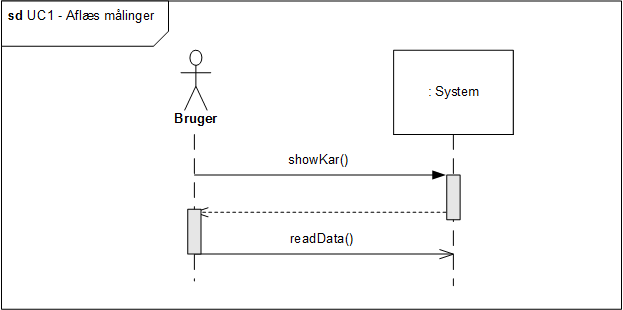
\includegraphics[width=0.8\textwidth]{Systemarkitektur/OverordnedeSekvensdiagrammer/sd_UC1.PNG}
    \caption{sd - Usecase 1}
    \label{fig:sd_UC1}
\end{figure}

\subsection{Overordnet sekvensdiagram for usecase 2 - Manuel vanding}
På diagrammet ses interaktion mellem System og Bruger for usecase 2 - Manuel vanding.

\begin{figure}[H]
    \centering
    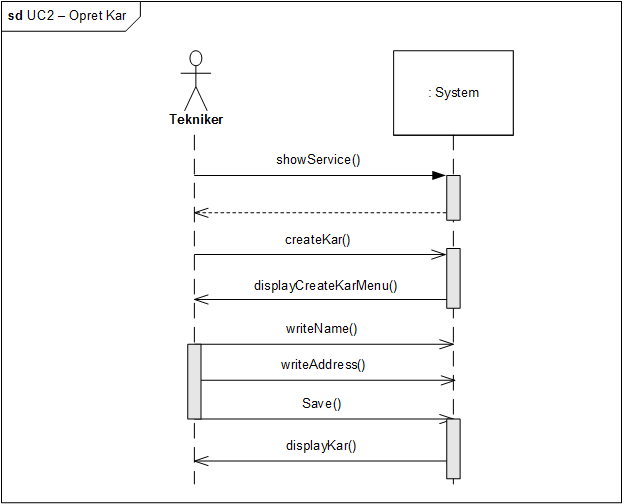
\includegraphics[width=0.8\textwidth]{Systemarkitektur/OverordnedeSekvensdiagrammer/sd_UC2.PNG}
    \caption{sd - Usecase 2}
    \label{fig:sd_UC2}
\end{figure}


\subsection{Overordnet sekvensdiagram for usecase 3 - Indtast pH-værdi}
På diagrammet ses interaktion mellem System og Bruger for usecase 3 - Indtast pH-værdi.

\begin{figure}[H]
    \centering
    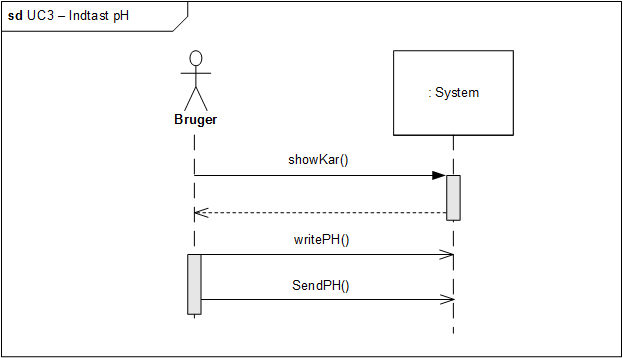
\includegraphics[width=0.8\textwidth]{Systemarkitektur/OverordnedeSekvensdiagrammer/sd_UC3.PNG}
    \caption{sd - Usecase 3}
    \label{fig:sd_UC3}
\end{figure}

\subsection{Overordnet sekvensdiagram for usecase 4 - Indtast volumen}
på diagrammet ses interaktion mellem System og Bruger for usecase 4 - Indtast volumen.

\begin{figure}[H]
    \centering
    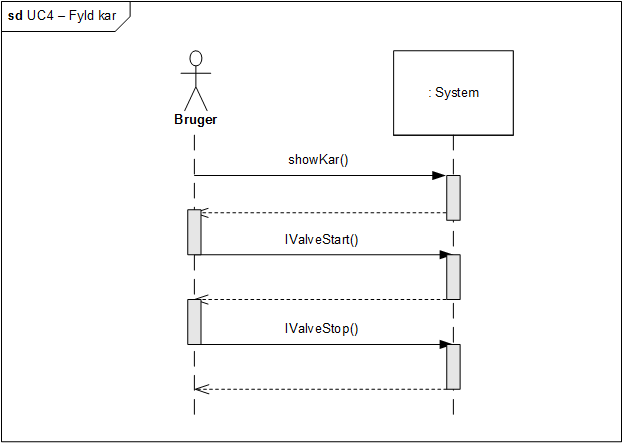
\includegraphics[width=0.8\textwidth]{Systemarkitektur/OverordnedeSekvensdiagrammer/sd_UC4.PNG}
    \caption{sd - Usecase 4}
    \label{fig:sd_UC4}
\end{figure}

\subsection{Overordnet sekvensdiagram for usecase 5 - Opret kar}
På diagrammet ses interaktion mellem System og Tekniker for usecase 5 - Opret kar.

\begin{figure}[H]
    \centering
    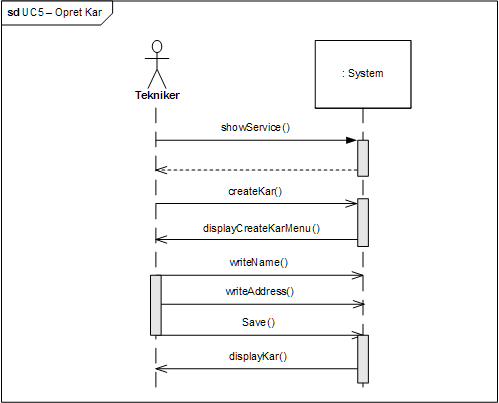
\includegraphics[width=0.8\textwidth]{Systemarkitektur/OverordnedeSekvensdiagrammer/sd_UC5.PNG}
    \caption{sd - Usecase 5}
    \label{fig:sd_UC5}
\end{figure}

\subsection{Overordnet sekvensdiagram for usecase 6 - Slet kar}
På diagrammet ses interaktion mellem System og Tekniker for usecase 6 - Slet kar.

\begin{figure}[H]
    \centering
    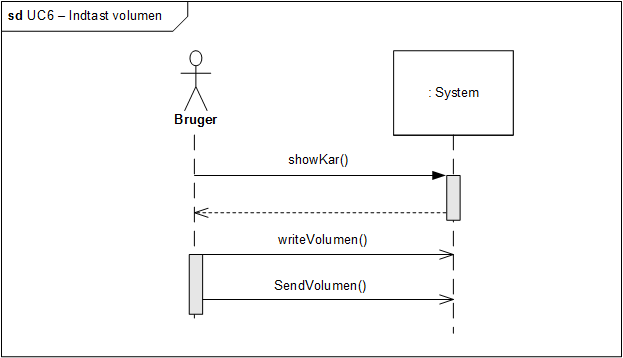
\includegraphics[width=0.8\textwidth]{Systemarkitektur/OverordnedeSekvensdiagrammer/sd_UC6.PNG}
    \caption{sd - Usecase 6}
    \label{fig:sd_UC6}
\end{figure}

\subsection{Overordnet sekvensdiagram for usecase 7 - Kalibrer pH-probe}
På diagrammet ses interaktion mellem System og Tekniker for usecase 7 - Kalibrer pH-probe.

\begin{figure}[H]
    \centering
    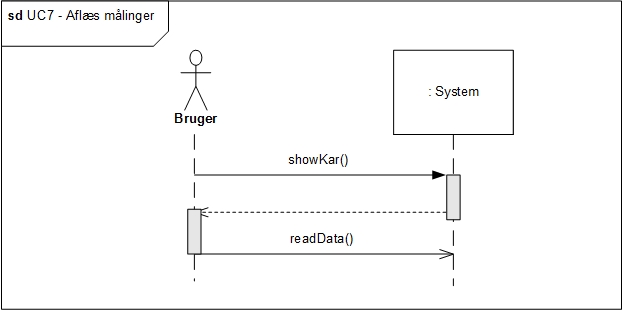
\includegraphics[width=0.8\textwidth]{Systemarkitektur/OverordnedeSekvensdiagrammer/sd_UC7.PNG}
    \caption{sd - Usecase 7}
    \label{fig:sd_UC6}
\end{figure}
